% Created 2015-07-09 dj 10:50
\documentclass[11pt]{article}
\usepackage[utf8]{inputenc}
\usepackage[T1]{fontenc}
\usepackage{fixltx2e}
\usepackage{graphicx}
\usepackage{longtable}
\usepackage{float}
\usepackage{wrapfig}
\usepackage{soul}
\usepackage{textcomp}
\usepackage{marvosym}
\usepackage{wasysym}
\usepackage{latexsym}
\usepackage{amssymb}
\usepackage{hyperref}
\tolerance=1000
\providecommand{\alert}[1]{\textbf{#1}}

\title{Curriculum  Vitae}
\author{Albert Baranguer Codina}
\date{\today}
\hypersetup{
  pdfkeywords={},
  pdfsubject={},
  pdfcreator={Emacs Org-mode version 7.9.3f}}

\begin{document}

\maketitle

\setcounter{tocdepth}{3}
\tableofcontents
\vspace*{1cm}

\section{Dades personals}
\label{sec-1}

\emph{Les meves dades personals bàsiques.}

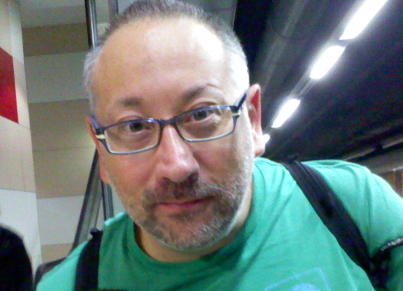
\includegraphics[width=.9\linewidth]{./img/albert_baranguer_codina_mq.png}

Albert Baranguer Codina

Nascut a Barcelona, 12 de desembre de 1968 (46 anys).

Casat i amb un fill.
\section{Formació universitària}
\label{sec-2}

\emph{Sóc Enginyer.}

Enginyer Tècnic de Telecomunicació. Especialitat Equips Electrònics.

1992: Escola Universitària Politècnica de Vilanova i La Geltrú, actualment \href{http://www.epsevg.upc.edu/}{Escola Politècnica Superior d'Enginyeria de Vilanova i la Geltrú}.

\href{http://www.upc.edu/?set_language=ca}{Universitat Politècnica de Catalunya}.
\section{Cursos i MOOC}
\label{sec-3}

\emph{M'agrada estudiar i aprendre.}
\subsection{MOOC}
\label{sec-3-1}

\emph{MOOC vol dir ``Massive Open Online Courses''.}
\subsubsection{MiriadaX}
\label{sec-3-1-1}

\emph{\href{https://www.miriadax.net/}{MiriadaX} és la plataforma MOOC hispana.}

MOOC: “Android: Programación de Aplicaciones” - Universitat Politècnica de València.

MOOC: “Curso Fundamental de Microeconomía” - Universidad Rey Juan Carlos de Madrid.

MOOC: ``Innotools 2na.ed. (Empathy Map - Business Model Canvas)'' - Universitat Pompeu Fabra - Fundació Tecnocampus.

MOOC: ``Introducción al Business Intelligence'' - Universitat Oberta de Catalunya (pràctiques amb llenguatge R).
\subsubsection{UNED-COMA}
\label{sec-3-1-2}

\emph{COMA vol dir “Cursos Online Masivos y Abiertos“. \hyperref[https-coma.uned.es]{UNED-COMA} és la plataforma MOOC de la UNED.}

MOOC: “La Contabilidad, el lenguaje de los negocios” - UNED-COMA.
\subsubsection{Coursera}
\label{sec-3-1-3}

\emph{\href{https://www.coursera.org/}{Coursera} és, probablement, la millor plataforma internacional de MOOC.}

MOOC: ``Digital Systems - Sistemas Digitales: De las puertas lógicas al procesador'' - Universitat Autònoma de Barcelona - Grade Achieved: 91.1\%

MOOC: ``Digital Signal Processing'' - École Polytechnique Fédérale de Lausanne - Grade Achieved: 72.8\% (pràctiques amb Octave, versió free open source software de Matlab, i Python).

MOOC: ``An Introduction to Financial Accounting'' - University of Pennsylvania - Grade Achieved: 75.4\%

MOOC: ``An Introduction to Marketing'' - University of Pennsylvania - Grade Achieved: 79.0\%

MOOC: ``An Introduction to Operations Management'' - University of Pennsylvania - Grade Achieved: 89.2\%

MOOC: ``Computing for Data Analysis (R Language)'' - Johns Hopkins University - Grade Achieved: 96.0\% with Distinction (pràctiques amb llenguatge R).

MOOC: ``Financial Engineering and Risk Management Part I'' - Columbia University - Grade Achieved: 85.7\%

MOOC: ``Financial Engineering and Risk Management Part II'' - Columbia University - Grade Achieved: 100.0\%

MOOC: ``Linear and Integer Programming'' - University of Colorado Boulder \& University of Colorado System - Grade Achieved: 73.3\% (pràctiques amb Octave, versió free open source software de Matlab).

MOOC: ``Introduction to Finance'' - University of Michigan - Grade Achieved: 100.0\%

MOOC: ``An Introduction to Interactive Programming in Python'' - Rice University - Grade Achieved: 85.8\%
\subsubsection{Stanford Online}
\label{sec-3-1-4}

\emph{\href{http://online.stanford.edu/}{Stanford} compta amb plataforma de MOOC pròpia.}

MOOC: “Finance“, per la Stanford University (Venture-Lab, actualment Stanford Online).
\subsection{Certificacions i formació postgrau}
\label{sec-3-2}

\emph{Postgrau de desenvolupament d'Aplicacions Internet.}

Master curs de postgrau de Desenvolupament d’Aplicacions Internet - Fundació Politècnica UPC.

03/06/2005 Homologació del curs de postgrau de Desenvolupament d’Aplicacions Internet - Indra - Fundació Politècnica).
\subsection{Formació Indra}
\label{sec-3-3}

\emph{Cursets realitzats dins l'àmbit del plà de formació de Indra.}

De 09/09/2013 a 25/09/2013 ``Flexibilidad y cambio'' (4 hores, Online).

De 02/04/2013 a 25/04/2013 ``Solventar los conflictos'' (6 hores, Online).

De 20/09/2010 a 08/10/2010 ``Autonomía y Decisiones en equipo'' (6 hores, Online).

De 19/10/2009 a 22/10/2009 ``SharePoint'' (16 hores, Versió reduïda del curset realitzat uns mesos abans).

De 07/10/2009 a 18/11/2009 ``ASP .Net'' (49 hores, Online).

De 07/10/2009 a 18/11/2009 ``C\# .Net'' (65 hores, Online).

De 19/01/2009 a 23/01/2009: Curset Advanced SharePoint
Impartit per \emph{GlobalKnowledge}. 30 hores.

De 02/06/2008 a 09/06/2008: Curset d’introducció a ABAP
Formació interna de Indra. 20 hores.

De 13/05/2008 a 22/05/2008. Curset d’introducció a SAP BW
Impartit per \emph{SAP Ibérica}. 48 hores.

De 28/11/2007 a 29/11/2007: Fonaments i tècniques de programació – Matlab
Impartit per \emph{The Mathworks}. 16 hores.

De 12/06/2006 a 16/06/2006: Curs de desenvolupament d’aplicacions web amb ContentServer FatWire
Impartit per \emph{Fatwire Ibérica}. Oficines de Fatwire Ibérica a Majadahonda. 40 hores.

De 08/05/2006 a 18/05/2006: Arquitectura, disseny i Aplicacions J2EE i Patrons de Disseny
Impartit per \emph{BIT FORMACIÓN INFORMÁTICA}. 32 hores.

De 01/11/2005 a 12/12/2005: Curs On-Line de Sun de Desenvolupament d'Aplicacions Java.

De 07/10/2002 a 17/10/2002: Desenvolupament i Arquitectura d’Aplicacions basades en .NET
Impartit per \emph{JJEC-FORMACIO, SL.L.}. 32 hores.

De 12/03/2001 a 22/03/2001: Desenvolupament d’aplicacions J2EE sobre iPlanet Application Server
Impartit per \emph{BIT FORMACIÓN INFORMÁTICA}. 32 hores.

De 16/11/2000 a 17/11/2000: Curs de Tècniques de preparació i direcció de reunions. (1 dia)
\section{Idiomes}
\label{sec-4}

\emph{Quines llengües parlo?}

Bilingüe català i castellà.

Anglès i francès: nivell mig-alt de conversa, comprensió i escrit.
\section{Experiència professional}
\label{sec-5}

\emph{Tinc un cert bagatge.}
\subsection{Experiència Professional a Indra}
\label{sec-5-1}


El darrer any he simultanejat manteniment i projectes entre Aigües de Barcelona i Gas Natural.
\subsubsection{de 01/10/2014 fins l'actualitat}
\label{sec-5-1-1}

Equip d'Arquitectura de Synectic (Grup Aigües de Barcelona).

Desenvolupament de l'aplicació d'Integració de Sistemes Comercials - \href{https://en.wikipedia.org/wiki/Society_for_Worldwide_Interbank_Financial_Telecommunication}{SWIFT} (Society for Worldwide Interbank Financial Telecommunication) del grup Aigües de Barcelona.

Aplicació basada en \textbf{Apache Camel} sobre servidor \textbf{JBoss Fuse} (Servidor Karaf OSGi) amb llenguatge Java. Integracio de l'aplicació al Framework d'Arquitectura d'Aigües de Barcelona (Maven, Repositori  maven corporatiu basat realitzat amb Nexus, Integració continua amb Jenkins, Qualitat de Codi amb SonarQUBE). 

L'objectiu del projecte és reemplaçar progressivament la integració de Sistemes Comercials amb Sistemes Bancaris via BizTalk i Editran per una solució basada en Apache Camel i SWIFT.

Suport al desenvolupament, proves i desplegament de l'aplicació FacturaE, basada en  \textbf{Apache Camel} sobre servidor \textbf{JBoss Fuse} seguint el Framework d'Arquitectura d'Aigües de Barcelona. 

Desenvolupament de web services amb \textbf{Apache Camel} sobre \textbf{JBoss Fuse} que reemplacen els web services equivalents desplegats sobre \textbf{Biztalk}. 

Responsable del manteniment i resolució d'incidències del servidor d'Integració \textbf{BizTalk 2006}, que gestiona les interfases entre diferents sistemes (comercials, financers, serveis, SAP ) interns i externs del grup Aigües de Barcelona.
\subsubsection{De 01/05/2014 fins 01/10/2014}
\label{sec-5-1-2}

Equip de Desenvolupament Web de Synectic (Grup Aigües de Barcelona)

\underline{Degut a la necessitat de suplir baixes de personal}, m'encarrego del manteniment i resolució d'incidències sobre \textbf{Lotus Notes}. Desenvolupo macros i codi en Lotusscript (llenguatge similar al VBA amb l'afegit d'objectes propis de Lotus Notes). 

\underline{Pel mateix motiu}, assumeixo manteniments i resolució d'incidències sobre webs corporatives implementades amb \textbf{LifeRay}.
\subsubsection{De 01/11/2007 fins l’actualitat}
\label{sec-5-1-3}

Equip JAVA del Servei GNI ECOFI.
\begin{itemize}

\item Des de 1 de maig de 2015\\
\label{sec-5-1-3-1}%
Migració de l'aplicació RiskManager de \emph{Java1.4, Framework GNI 2006,  Weblogic8.1, SGBD Oracle9, SO Windows Server}  a  \emph{Java7, Framework GNI 2010, Weblogic12c, SGBD Oracle12c, SO Linux Red Hat}.

M'encarrego de les adaptacions, i validació bàsica de funcionament de l'aplicació amb la nova arquitectura  i del seu desplegament.

Previst que m'ocupi del desenvolupament de part de les noves funcionalitats.


\item Desembre de 2014\\
\label{sec-5-1-3-2}%
S'abandona el manteniment de la NaturalNet.


\item Des de 1 de gener de 2012\\
\label{sec-5-1-3-3}%
M'afegeixo a l'equip de manteniment del Risk Manager. Aplicació Web de parametrització d'escenaris per a simulació de risc de crèdit. (Java 1.4, Weblogic 8.1, Spring, PL/SQL Oracle 9. Motor de càlcul de simulacions fet amb Matlab). S'assumeix el manteniment i desenvolupament de la aplicació Standalone Java Swing ``Ventana KE''. Una aplicació de la família del Risk Manager que permet configurar simulacions específiques de capital econòmic que són executades amb el motor de càlcul Matlab del Risk Manager.    

S'afegeix el manteniment de la NaturalNet (Intranet de Gas Natural). SharePoint. Gestió de continguts i, eventualment, desenvolupaments en MOSS.

S'abandona el manteniment del ``Portal Corporativo'' i les aplicacions Java EE del ``Portal Corporativo''. 

S'abandona el manteniment del ``Portal de la Fundación de gas Natural''.


\item Des de 1 de gener de 2010\\
\label{sec-5-1-3-4}%
Manteniment de l'aplicació web SIRCA (Risc de crèdit) (Framework SEAM 2.0, Java j2ee) i de les aplicacions batch standalone (realitzades en java) de càrrega de puntuacions. Mantenimient dels processos PL/SQL de puntuacions.


\item Des de 1 de gener de 2009.\\
\label{sec-5-1-3-5}%
Continuo amb els manteniments heretats de l’etapa anterior: Factura Web de Gas Natural i Web de WorkFlows.

S’afegeix manteniment del Portal Corporatiu de GasNatural (Fatwire), i de les aplicacions j2ee del portal: Curricula (inserció de CV externs), Emailing Corporatiu (accions d’emailing), Clickthrough (comptador de clicks en banners), Arxiu Audiovisual (gestor de media), i Productes Homologats (aplicació d’un intern per al control de versions de software corporatiu). A més, també s’assumeix el manteniment del sistema j2ee SIC Sistema d’Informació de Qualitat) per control de qualitat de les visites d’inspecció (Java 1.4, Weblogic 8.1, Spring, PL/SQL Oracle 9).

S'afegeix el manteniment (gestió de continguts i desenvolupaments en MOSS) del ``Portal de la Fundación de Gas Natural'' en SharePoint.


\item De 01/10/2008 a 01/11/2008\\
\label{sec-5-1-3-6}%
Realització d’informe amb Excel, SAPEx Analyzer i Reports amb QueryDesigner de SAP-BW, per al projecte CFM de GasNatural.


\item De 01/02/2008 a 31/12/2008.\\
\label{sec-5-1-3-7}%
Pas a producció, manteniment i evolutius de la Factura Web. Manteniment i evolutius de web de workflows (inclosa web de wf de Propuestas de Inversión (PI) - Propuestas de Contratación de Asesoría Externa (PCAE)).


\item De 01/11/2007 a 01/02/2008\\
\label{sec-5-1-3-8}%
Desenvolupament mòdul de conversió XML a PDF amb Apache FO (Formatting Objects) de la Plataforma de Facturació Electrònica de Gas Natural. Java, Servlets, FO, XML, XSL. 

Subversion, Metodologia iterativa.


\item De 01/08/2007 a 01/11/2007\\
\label{sec-5-1-3-9}%
Desenvolupament d’aplicació frontend web per a l’aplicació de WorkFlows de Propostes d’Inversió i de Propostes de Contractació d’Auditoria Externa de Gas Natural (WF-PIPCAE). Java, Servlets, DHTML, Javascript, MQ, Subversion, Metodologia iterativa.

Desenvolupament de mòdul de Propostes de Provisió per al frontend web de l’aplicació de Gestió de WorkFlows Econòmics-Financers de Gas Natural. Java, Servlets, DHTML, Javascript, MQ, Subversion, Metodologia iterativa

\end{itemize} % ends low level
\subsubsection{De 01/02/2005 fins 01/11/2007}
\label{sec-5-1-4}

Manteniment sistemes SGO-GNS y SGO-GNCOM de Gas Natural. Arquitectura J2EE. Patró Model View Controller. Oracle 9i. 

Desenvolupament d’scripts PL/SQL, Java, DHTML, Javascript, CSS, XSTL, XML, Apache POI, JFreeChart, Framework MVC de GNI (SGO-GNS) , Framework propietari AIA (SGO-GNCOM) , Eclipse , TOAD. BEA Weblogic Application Server 8.1 Java, Servlets, DHTML, Javascript, MQ, CVS Subversion, Metodologia iterativa
\subsubsection{De 16/08/2004 a 01/02/2005}
\label{sec-5-1-5}

Sistema SGO-GNS de Gas Natural Arquitectura, disseny i desenvolupament.

Arquitectura J2EE, patró Model View Controller. Oracle9i. Scripts PL/SQL, Framework MVC de GNI, Java. DHTML, Objectes Apache POI (java – excel), Javascript, CSS, JSP, Eclipse, TOAD. BEA WebLogic Application Server 8.1,CVS, metodologia iterativa.
\subsubsection{De 01/03/2004 a 30/06/2004}
\label{sec-5-1-6}

Media Asset Management.

Media Asset Management per a Retevision Abertis (projecte de Grupo Delaware).

Disseny i desenvolupament, Arquitectura J2ee, Oracle, Plataforma MVC eCompany Gaudí d’Auna – Abertis, Java, DHTML, Javascript, Jbuilder, TOAD, BEA Weblogic Application Server 6.1. Source Safe, metodologia iterativa.
\subsubsection{De 01/02/2004 a 01/03/2004}
\label{sec-5-1-7}

Interfase del Sistema de Provisionament Logístic.

Interfase del sistema de provisionament logístic per a Retevision Abertis (projecte de Grupo Delaware).

Disseny i desenvolupament,  Arquitectura J2ee, Oracle, Plataforma MVC eCompany Gaudí d'Auna – Abertis, Java, DHTML, Javascript, Jbuilder. TOAD. BEA Weblogic Application Server 6.1, Source Safe, metodologia iterativa.
\subsubsection{De 01/07/2003 a 01/02/2004}
\label{sec-5-1-8}

Sistema ISIS. Anàlisi i correcció de processos de càrrega.

Participo al projecte conjunt Indra Sistemas-SoluZiona de desenvolupament del sistema ISIS d’integració d’informació operacional, basada en l’estàndar SID (Shared Information Data) d’NGOSS (New Generation Operation Systems and Software) del Telemanagement Forum. 

En el sistema s’integra informació operacional (dades quasi-crues) provinents de diversos sistemes de les operadores de cable del grup Auna amb informació provinent de sistemes de RETEVISION. 

Participo en l’anàlisi del bloc de Provisió de Serveis i Inventari i Construcció de Xarxa, i també en el desenvolupament d’scripts de càrrega (Processos ETL extracció - transformació - càrrega) i reparació de dades. Oracle PL-SQL, Transact-SQL de Sybase, Scripts shell unix, TOAD.
\subsubsection{De 01/04/2003 a 01/07/2003}
\label{sec-5-1-9}

Extracció de dades de grans clients.

Disseny i desenvolupament de l’extracció de dades de grans clients del sistema CRM de RETEVISION enriquits amb dades del Sistema de Provisió. Interfase d’enviament d’aquest paquet de dades a Auna Grandes Clientes, mitjançant canal segur SCP i automatització de tot el procés mitjançant Control-M. PL/SQL i Korn Shell. Oracle, TOAD, PLSQL Developer, SCCS, metodologia en cascada.
\subsubsection{De 01/02/2003 a 01/04/2003}
\label{sec-5-1-10}

Gestió d’interfases del CRM d’Auna Grandes Clientes.

Disseny i desenvolupament. El sistema controla les transmissions de fitxers entre diferents sistemes d’Auna Telecomunicaciones (Amena + Retevisión) al CRM d’Auna Grandes Clientes. 

Weblogic Application Server 5.1. Java, JSP, Servlets, PL/SQL Oracle 9i, SourceSafe, metodologia iterativa
\subsubsection{De 01/11/2002 a 01/02/2003}
\label{sec-5-1-11}

Extracció de contractes del CRM Vantive.

Pla de proves, Disseny i desenvolupament. Migració de bases de dades del sistema d’extracció de contractes del CRM Vantive de RETEVISION. Desenvolupo el pla de proves i els scripts de proves. Modificació d’Scripts d’extracció Korn Shell, Perl i Transact-SQL de Sybase. Disseny i desenvolupament de servlets d’extracció sobre iPlanet Application Server 6.1. SCCS, metodologia en cascada
\subsubsection{De 01/08/2002 a 01/11/2002}
\label{sec-5-1-12}

Projecte TITAN.

Disseny i desenvolupament d’utilitats diverses per al projecte TITAN (Migració del catàleg de disseny de les centrals d’entorn host a entorn micro) de l’ANAV (Agrupació Nuclear Ascó Vandellós). 

Desenvolupo l’eina de generació d’esquemes XSD per a les consultes SQL-XML en SQL Server 2000. 

Disseny del mòdul d’impressió de fitxes. Visual Basic 6.0. XSDSchema per a Sql Server 2000, Soap Toolkit de MS, SourceSafe,  metodologia iterativa
\subsubsection{De 01/06/2002 a 01/07/2002}
\label{sec-5-1-13}

Provisió de serveis Internet (mòduls del Sistema de Provisió de Serveis).

Disseny, desenvolupament. evolutius i correctius.Participo al projecte PINET (Provisió de serveis Internet) de NET per a Retevision. 

Anàlisi, disseny, desenvolupament, posada en produccuó, manteniment i evolutius del subprojecte de ISPs Virtuals. Plataforma J2EE: Servidor Web iPlanet, Servidor d’Aplicacions Aplicaciones iPlanet. HTML, JavaScript, Servlets, JSP, EJBs, PL-SQL, Source Safe, metodologia iterativa.

Indra s’encarrega del manteniment i desenvolupament de PINET. Posteriorment l’equip de PINET es fusiona amb altres equips per a formar el gruix de l’equip de desenvolupament del Sistema de Provisió de Serveis (SPS) de Retevision.

Disseny del servei web de interfase entre SPS i plataformes de contractació. Disseny del servlet de interfase i missatgeria.

Anàlisi, disseny i desenvolupament de Versió II i III de la web de ISPs virtuals. Source Safe. Metodologia iterativa.Anàlisi, disseny i pilot de web d’autoprovisió.

Disseny i desenvolupament de provisió de productes “ADSL Marca Blanca'', metodologia en cascada, Arquitectura J2ee, Oracle, PL/SQL, Java DHTML, Javascript. XML, Source Safe.

Manteniment i provisió del sistema d’ISPs virtuales de Caixa Catalunya, metodologia en cascada, Arquitectura J2ee, Oracle, PL/SQL, Java DHTML, Javascript. XML, Source Safe.
\subsubsection{De 01/04/2000 a 01/06/2000}
\label{sec-5-1-14}

Control de facturació GasNatural.

Suport al desenvolupament del projecte de control de facturació en Visual Basic 5.0 de Gas Natural SDG.

Visual Basic 5.0 BD Multidimensional Hyperion EssBase. Oracle. VBA per Excel. Source Safe. Metodología iterativa
\subsubsection{Del 01/07/1999 al 01/04/2000}
\label{sec-5-1-15}

Sistema de Transmissió i Control d‘Interfases (STCI) del Grupo ENDESA.

Disseny i desenvolupament de la segona fase del STCI. 

Desenvolupament de Serveis Windows amb Visual C++, visualització d’alertes al visor d’events de Windows, accés al registre de Windows per a configuració dels serveis, Oracle, mòduls d‘Intranet sobre MS Internet Infomation Server amb ASP i Visual Interdev 6.0, desenvolupament d’utilitats de càrrega i manteniment de taules i de control dels servei, source safe, Metodologia en cascada
\subsection{Experiència Professional anterior}
\label{sec-5-2}
\subsubsection{De 01/05/1999 a 01/07/1999}
\label{sec-5-2-1}

\textbf{LEVELDATA SCA}
Projecte de Datawarehouse de trucades de Indra Sistemas per a Retevisión. 

Disseny i desenvolupament de l’aplicació de manteniment de taules del sistema (Visual Basic 5.0 i Oracle). Amb aquest projecte deixo Level Data i entro a Indra Sistemas (maig 1999).

Arquitectura client servidor. Oracle, VB5, metodologia iterativa.
\subsubsection{De 01/12/1998 a 01/05/1999}
\label{sec-5-2-2}

\textbf{LEVELDATA SCA}
Primera fase del projecte de Indra Sistemas per a Endesa del Sistema de Transmissió i Control d‘Interfases (STCI).

Desenvolupo DLL de connexió de clients NT al sistema amb Visual C++, mòduls d’Intranet de control del sistema amb ASP i Visual Interdev 1.0 i consultes a BD Oracle, metodologia iterativa.

Professor de curset de Programació en Java de formació Interna a Level Data. (Aprox. de 40h) . Metodología de desenvolupament en cascada

\emph{Fins el moment d’entrar a LevelData la meva activitat professional es desenvolupava en règim de pluriempleat, amb l’activitat de professor associat a temps parcial a l’Escola Univeritària de Mataró com tasca principal}.
\subsubsection{Del 01/01/1998 al 01/12/1998}
\label{sec-5-2-3}

\textbf{CDLAB}
programador de la web, bd i aplicació de consulta standalone de la ``Guía electrónica España 30000'' amb dades de 30000 empreses estatals. Access,Active Server Pages i SQL Server, Visual Interdev, Delphi 1.0. Metodologia en cascada.
\subsubsection{Del 01/01/1997 al 01/01/1998}
\label{sec-5-2-4}

\textbf{Sercolan (Holzadac S.L.)}
Projecte de nova empresa que pretenia crear un portal web per al sector de la construcció. 

Access, CGI amb perl sobre servidor Web Apache, Linux.
\subsubsection{Del 01/06/1996 al 01/12/1998}
\label{sec-5-2-5}

\textbf{Editorial Cypsela S.L}
Revista Electrónica \& Comunicaciones Magazine. Manteniment dels equips informàtics.

Desenvolupo el software de “Guía de Tiendas de Electrónica” que es va incloure l’estiu del 98 amb la la guía en paper “Las Tiendas”. 

Delphi 1 (Object Pascal), disseny, desenvolupament i manteniment de la Web de Cypsela S.L. metodologia en cascada. 

De forma esporàdica publico algun article tècnic a la revista.
\subsubsection{De 01/01/1996 a 01/01/1997}
\label{sec-5-2-6}

\textbf{Institut Joan Pelegrí d’Hostafrancs}
Per substitució d’una baixa per maternitat, a l’Institut Joan Pelegrí de Hostafrancs:

Professor de Batxillerat Tècnic i FP. Imparteixo cursos de C, Pascal i Access.

Professor de mòdul professional de grau superior de Disseny d’Aplicacions Informàtiques.
\subsubsection{De 01/11/1992 a 01/12/1998}
\label{sec-5-2-7}

\textbf{Escola Universitària Politècnica de Mataró}
Professor associat a temps parcial a l’Escola Universitària Politècnica de Mataró. 

Durant els sis anys passats allí desenvolupo la tasca de professor de pràcticas en qüestions molt diverses: 

Electrònica analògica (de 2n i 3er de telecomunicacions), instrumentació (3er telecomunicacions), teoria de circuits (2on industrials i telecomunicacions); transmissió d’ones (microones, antenes i fibra òptica) de 3er de telecomunicacions; Sistemes Operatius (Unix - Linux, C, C++, Shell Script, awk) de 2on telemàtica. Projectes (part de projectes d’aplicacions a Internet HTML, CGI, JavaScript, Java) de 3er telecomunicacions. Estructura de computadors (assembler 8086) de 1er informàtica de gestió.

A més, també soc professor ponent de projectes de final de carrera.
\subsubsection{De 01/06/1992 a 01/11/1992}
\label{sec-5-2-8}

\textbf{SIC Informática}, de Granollers.
Programador auxiliar, 4GL i SQL de Informix sobre SCO unix.
\section{Aficions}
\label{sec-6}

\emph{A la vida no tot és feina.}

Soc blocaire. M'agrada escriure. Això ho combino amb un gran interès per la política i l'activisme social, per una banda; i també interès per la tecnologia. El resultat és que mantinc un parell de blocs:

\href{http://www.albertbaranguer.cat/?m=1}{El Blog d'Albert Baranguer}

\href{http://stsoftlliure.wordpress.com}{Apunts de Tecnologia}

Però no em passo la vida enganxat a un teclat. També m'agrada fer excursions a peu, o en bici.
\section{Publicacions}
\label{sec-7}

\emph{Fins i tot he escrit un llibre! (o, si més no, alguns capítols).}

Diversos Articles tècnics a la revista Electónica y Comunicaciones Magazine.

Diversos capítols de ``Manual para Instaladores S.A.T, Editorial Cypsela S.L''. Albert Baranguer, Lluís Ibáñez, Jordi Pallarés, Xavier Prades i Mònica Gálvez.
\section{Dades de contacte}
\label{sec-8}

\emph{On em podeu trobar?}

\textbf{Adreça}:

c/ Sugranyes, 39-41, 3er-4t

08028 Barcelona

\textbf{Telefons}:

Tel.: 675 474 942

Fix : 93 332 44 18

\textbf{Internet}:

\emph{email}: \href{mailto:abaranguer@gmail.com}{mailto:abaranguer@gmail.com}

\emph{LinkedIn} \href{https://es.linkedin.com/pub/albert-baranguer-codina/26/797/900}{https://es.linkedin.com/pub/albert-baranguer-codina/26/797/900}

\emph{GitHub} \href{https://github.com/abaranguer}{https://github.com/abaranguer}
\section{Expectatives professionals}
\label{sec-9}

\emph{Què vull ser quan sigui (més) gran?}

El món en que vivim té grans reptes plantejats, com són el canvi climàtic o l'escassedat energètica, que poden provocar un retrocés en la qualitat de vida, drets i llibertats democràtiques de la majoria si no som capaços de donar respostes eficaces, intel·ligents i ètiques. 

Penso que el sector de les TI ofereix una part de les respostes als reptes plantejats: les smart cities, les smart grids, les fog-networks (el cloud a nivell de dispositius), l'e-democracy, els nous materials, l'eficiència energètica dels dispositius\ldots{} 

Aleshores, el meu objectiu és contribuir a les respostes de les TI als reptes plantejats. Participant en projectes i aprofitant l'oportunitat d'aprendre continuament. 

Em veig formant part d'equips de projecte, ja sigui liderant equips, o col·laborant en la definició de les arquitectures dels projectes, o col·laborant directament en el desenvolupament, i aportant en tots els casos la meva experiència diversa, humana, professional i docent.
\section{Com he fet aquest curriculum?}
\label{sec-10}

\emph{El format d'aquest CV em recorda alguna cosa\ldots{}}

He desenvolupat aquest curriculum fent servir l'org-mode d'Emacs i, a continuació, exportant a pdf, html i format freemind des del mateix Emacs.

Remarcar que la versió en pdf s'ha obtingut en dues passes: exportant, primer, a \LaTeX{}; i generant el pdf, després, amb pdflatex. 

L'exportació bàsica de l'org mode fa servir el format Report de \LaTeX{}, per això el format clàssic obtingut que recorda al de tants manuals que es troben a Internet. 

La versió freemind l'he exportat fent servir l'eina homònima a format flash. El resultat és un mindmap amb el meu CV que és navegable, ampliable, reduïble, col·lapsable\ldots{}

Tot plegat partint del simple codi font en org.

He desat el codi font del CV i les diferents conversions obtingudes al meu github.

\end{document}
